\documentclass[onecolumn, draftclsnofoot,10pt, compsoc]{IEEEtran}
\usepackage[utf8]{inputenc}
\usepackage[table,xcdraw]{xcolor}
\usepackage{graphicx}
\usepackage{tabularx}

% A one to two page document stating user stories
% Requirement example: a user must be able to learn how to use the web press from a remote location
% Don't really need any reference to VR here; that is more of a design choice than a requirement
% Concise; just whatever are the literal requirements that our project must fulfill
\title{Client Requirements Document Rev 2}
\author{Stephen Hoffmann, Stewart Rodger, Nicholas Pugliese, Kyle Tyler, Symon Ramos}
\date{October 2018}
\newpage

\begin{document}
\setlength\parindent{0pt}
\maketitle

\section*{Revisions}

\begin{table}[ht!]
\begin{tabularx}{\textwidth}{|l|X|X|}
\hline
\rowcolor[HTML]{C0C0C0} 
Section & Original & New \\ \hline
Specific Requirements &  HP needs a less expensive way to train Web Press customers on its operation and maintenance. These customers must receive training that prepares them for the operation and maintenance of the HP Web Press at the same level of competency as the in-person training seminars at an HP Web Press location. Creating an entire training program to replace the current system is not within the scope of this project. Instead, this project will focus on laying the groundwork for a training program and creating a single training scenario that can be used to show the worth of a virtual reality training program.    & Creating an entire training program to replace the current system is not within the scope of this project. Instead, this project will focus on laying the groundwork for a training program and creating a single training scenario that can be used to show the worth of a virtual reality training program.   \\ \hline
\end{tabularx}
\end{table}

% What are a few things that are fundamental to the program?
% What is the big idea -> user needs to learn web press remotely
\section{General Requirements}
There is a need for personnel and HP customers to be trained on HP's Web Press printers. The current methodology of training requires extensive resources in order to fly customers to a location with an HP Web Press, provide food and a hotel rooms for the duration of the training, and halt any production on the Web Press while the training exercises are running. The current training method also can't account for cases where the Web Press breaks because it's not applicable to break a Web Press for the sole purpose of teaching personnel how to react in that scenario.

% What are some requirements specific to a certain part of the project?
\section{Specific Requirements}
HP needs a less expensive way to train Web Press customers on its operation and maintenance. These customers must receive training that prepares them for the operation and maintenance of the HP Web Press at the same level of competency as the in-person training seminars at an HP Web Press location. Creating an entire training program to replace the current system is not within the scope of this project. Instead, this project will focus on laying the groundwork for a training program and creating a single training scenario that can be used to show the worth of a virtual reality training program. 

% Inputs/Outputs -> need computer, some kind of input device, visual output
% \subsection{External interfaces}
The customer must have access to facsimiles or analogs of the HP Web Press technology in order to gain familiarity with the real product. When they use a real Web Press for the first time after the remote training they must feel familiar with the physical hardware.

Customers with no prior industrial printing experience should be able to complete the training with adequate knowledge retention.
% Measurable effectiveness
% Efficiency
% Satisfaction criteria in specific contexts of use
% \subsection{Usability}

% Frame rate
% Number of simultaneous users supported
% Load times
% I think performance (and other non-functional requirements) are a design document item, not solution requirements -N
%\subsection{Performance}

The new training program must also be more preferable by HP than their old training program and cause them to consider adopting this new method instead.

% Constraints on the program imposed by external standards, regulatory requirements, or project limitations
% Ex: OS constraints, memory, etc
\subsection{Constraints}
The training program should be significantly less expensive per customer to complete than the current in person training model. Ideally there should be no transportation or food expenses to account for. The customer should not have to leave their home or place of business to complete the training. It should be accessible to customers anywhere in the world that has an internet connection. The solution should only include existing HP products utilize preexisting business agreements HP possesses with current technology leaders. 

\section{Gantt Chart}
\bigskip
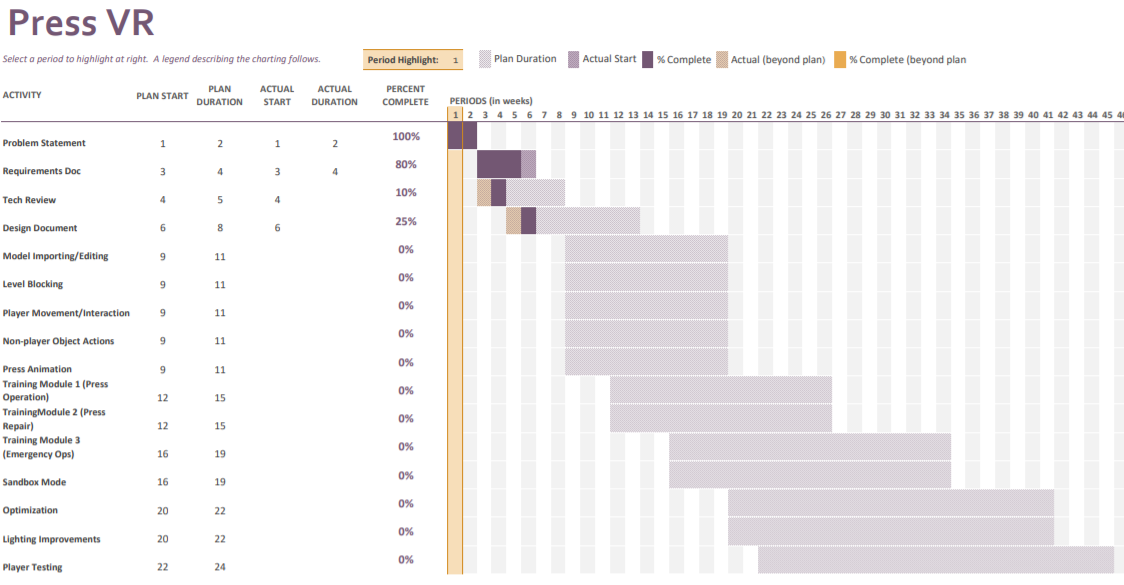
\includegraphics[scale=.75]{ganttChart.PNG}


\end{document}
